\section{Controller}
The controller is responsible for stabilizing the rocket state, attenuating any disturbances, and driving it to some desired value.
In their configuration the canards can only provide a torque around the roll ($x$) axis of the rocket.
This imposes some constraints on the controller design, as the whole state \ref{eq:model-state-vector} is under-actuated.
The model used for controller design is thus simplified to the state \ref{eq:controller-model-state}, using a linear parameter-varying system.

The controller chosen for the canards is linear state feedback, where the feedback gains $K$ are computed by the \textit{Linear Quadratic Regulator} (LQR) method \cite{werner2021, werner2021b}.
The current state is determined by the state estimation algorithm (the Estimator is treated in Section \ref{sec:estimator}), as seen in Figure \ref{fig:controller-loop}.
The loop is a two-degree-of-freedom design, where the reference signal is prescaled by a feedforward (reference) gain $K_{pre}$.
To account for the non-linearity of the rocket dynamics the gains are selected from a gain schedule, which is a look-up table of gains for different parameters of the linear model from Equations \ref{eq:controller-model-state}, 
\ref{eq:controller-model-ss}, and \ref{eq:controller-model-matrices}. 

\begin{figure}[ht]
    \centering
    \resizebox{0.8\textwidth}{!}{
    \newcommand\lw{0.75pt}
% style of elements
\tikzstyle{block} = [draw, fill=white!20, rectangle, 
    minimum height=3em, minimum width=4em, line width = \lw]
\tikzstyle{dblock} = [draw, rectangle, 
    minimum height=4.5em, minimum width=16em, line width = \lw]
\tikzstyle{sum} = [draw, fill=white!20, circle, node distance=1cm, line width = \lw, inner sep = 0.075cm]
\tikzstyle{bullet} = [draw, fill=black!100, circle, node distance=1cm, line width = \lw, inner sep = 0.04cm]
\tikzstyle{input} = [coordinate]
\tikzstyle{output} = [coordinate]
\tikzstyle{branch} = [coordinate, bullet]
\tikzstyle{pinstyle} = [pin edge={to-,thin,black}]


\begin{tikzpicture}[auto, node distance=2.1cm,>=latex']
    % We start by placing the blocks
    \node [input, name=input] {};
    \node [block, right of=input, 
    node distance=3cm] (prescale) {$K_{pre}$};
    \node [sum, right of=prescale, xshift = 1cm] (sum) {};
    \node [branch, right of=sum, xshift = 1cm] (b1) {};
    \node [block, right of=b1, 
    		node distance=2.5cm] (plant) {Rocket};
    \node [branch, right of=plant, xshift = 2cm] (b2) {};
    \node [block, below of=plant, 
    		node distance=2.5cm] (observer) {Estimator};
    \node [block, left of=observer, 
    		node distance=3cm] (feedback) {$K$};
    \node [block, below of=feedback, 
    		node distance=2cm] (scheduler) {Schedule};
    \node [output, right of=b2, xshift = -1cm] (o1) {};

    \node [output, below of=plant, yshift = 0.8cm] (u_line1) {};
    \node [output, right of=observerxshift = -1cm, below of=plant, yshift = 0.8cm ] (u_line2) {};


    % Once the nodes are placed, connecting them is easy. 
    \draw [->, line width = \lw] (input) -- node {$r(t)$} (prescale);
    \draw [->, line width = \lw] (prescale.east) |- (sum);
    \draw [-, line width = \lw] (sum) -- node[pos=1] {$u(t)$}  (b1);
    \draw [->, line width = \lw] (b1.east) |- (plant);
    \draw [-, line width = \lw] (plant.east) |- (b2);
    \draw [->, line width = \lw] (b2) -- node[pos=0] {$y(t)$} (o1);
    \draw [->, line width = \lw] (b2) |- (observer.345);
    \draw [->, line width = \lw] (observer.west) -- node {$\hat x_R(t)$}(feedback);
    \draw [-, line width = \lw] (b1) |- (u_line1);
    \draw [-, line width = \lw] (u_line1) -- (u_line2);
    \draw [->, line width = \lw] (u_line2) |- (observer.15);
    \draw [->, line width = \lw] (feedback.west) -| (sum.south);
    \draw [->, line width = \lw] (observer.south) |- node[above,pos=0.7] {$\hat x_{FC}(t)$}(scheduler.east);
    \draw [->, dashed, line width = \lw] (scheduler.north) -- node {}(feedback.south);
    \draw [->, dashed, line width = \lw] (scheduler.west) -| node {}(prescale.south);

\end{tikzpicture}
}
    \caption[Block diagram of the control loop]{Block diagram of the control loop. 2-DOF estimator-based state feedback \cite{werner2021} with gain scheduling.}
    \label{fig:controller-loop}
\end{figure}

\subsection{Controller roll model}
\label{sec:controller_model}
The dynamic pressure and the canard coefficient $C_L$ are the scheduling variables of the controller.
The concocted state $x_R$ for the roll model (Equation \ref{eq:controller-model-state}) and the flight condition (Equation \ref{eq:controller-model-fc}) are
\begin{align}
    x_R &= \begin{bmatrix} \phi & \omega_x & \delta \end{bmatrix}^T 
    & 
    x_{FC} &= \begin{bmatrix} \bar p & C_L \end{bmatrix}
    \nonumber
\end{align}
The state-space model is (Equations \ref{eq:controller-model-ss})
\begin{align}
    \dot x_R &= A \: x_R + B \delta_u 
    &
    y_R &= C x_R
    \nonumber
\end{align}
with the matrices (Equations \ref{eq:controller-model-matrices})
\begin{align}    
    A(x_{FC}) &= \begin{bmatrix}
        0 & 1 & 0 \\
        0 & L_{\omega_x} & L_\delta \\
        0 & 0 & -\alpha
    \end{bmatrix}
    &
    B &= \begin{bmatrix}
        0 \\ 0 \\ \alpha
    \end{bmatrix}
    &
    C &= \begin{bmatrix} I_3 \end{bmatrix}
    \nonumber
\end{align}
where the roll control derivative is $L_\delta (\bar p,  \,  C_L)$, and the roll damping derivative is $L_{\omega_x} (\bar p, \, C_{L \omega_x})$.
The matrix $C$ combines the states of the system to an output signal, and can be set arbitrarily for response analysis.
For the case $C = \begin{bmatrix} I_3 \end{bmatrix}$, the output signal is the entire state vector $y(t) = x(t)$, for the case $C = \begin{bmatrix} 1 & 0 & 0 \end{bmatrix}$, the ouput signal is $y(t) = x_1(t) = \phi$.

The open-loop eigenvalues are simply
\begin{align}
    \lambda_1 &= 0 & \lambda_2 &= L_{\omega_x} & \lambda_3 &= -\alpha 
\end{align}
The rocket in open-loop is only marginally stable due to the free integrator from the roll rate to roll angle ($\omega_x \to \phi$).
Additionally, when using a spin can the damping derivative $L_{\omega_x}$ is very small compared to the control derivative $L_\delta$. 
When assuming $L_{\omega_x} \approx 0$ the open-loop is quadratically unstable.


\subsubsection{Controllability}
The (approximately in continuous time) closed loop is 
\begin{align}
    \dot x_R &= (A+BK) x_R + B K_{pre} r & y_R &= C x_R
    \label{eq:controller-closedloop}
\end{align}

To determine if pole placement is possible, which is a necessary condition for LQR \cite{werner2021}, the roll model is checked for controllability.
The controllability matrix is 
\begin{align}
    \mathcal{C} = \begin{bmatrix}
        B & AB & A^2 B 
    \end{bmatrix}
\end{align}
which has full rank for all $L_\delta \neq 0$, i.e. there exists a feasible feedback gain for every flight condition, except for zero velocity ($\lVert v \rVert = 0$) or a zero coefficient of lift ($C_L = 0$).

\subsection{Control law and tuning}

To compute the desired canard angle $u = \delta_u$, the the current rocket roll state as determined by the state estimation is used.
The control law is a state feedback, combined with a feedforward part for the reference signal $r$ as
\begin{align}
    u(t) &= K \hat x_R(t) + K_{pre} r(t)
\end{align}
where the gains $K = \begin{bmatrix} K_\phi & K_{\omega_X} & K_\delta \end{bmatrix}$ are determined by performing the LQR method around a linear model
\begin{align}
    K(\hat x_{FC}) &= -\texttt{lqr}(A(\hat x_{FC}),B,Q_{c},R_{c}) 
\end{align}
with Matlab's \texttt{lqr} function. 
For the discrete controller, the function \texttt{lqrd}($A, B, Q, R, dt$) is used to directly account for discrete dynamics with sampling time $dt$, but using a continuous-time system (A,B). 
To note: for fast sampling times (much higher sampling frequency than the bandwidth of the model), the feedback gains of \texttt{lqr} and \texttt{lqrd} become approximately equal.
The method is tuned by adjusting the weighting matrices $Q_c$ and $R_c$.
As shown in section \ref{sec:controller-theory}, the matrix $Q_c$ contains the weights for penalizing the state error, while the matrix $R_c$ weighs the expended control effort.

The scalar reference gain $K_{pre}$ is computed for a steady state gain of 1, as
\begin{align}
    K_{pre} (\hat x_{FC}) &=  \frac{-1}{C \left[ A(\hat x_{FC}) + B K(\hat x_{FC}) \right]^{-1} B}
\end{align}
where $C$ depends on the variable to be tracked. 
With $C = \begin{bmatrix} 1 & 0 & 0 \end{bmatrix}$, the channel $r \to \phi$ is selected, which results the roll angle tracking the reference.
The channel $r \to \omega_x$ could also be selected via $C = \begin{bmatrix} 0 & 1 & 0 \end{bmatrix}$, this would result in tracking of the roll rate.

The gains $K$ and $K_{pre}$ can be precomputed for each combination of parameters $A(\hat x_{FC})$.
As gain scheduling is used to account for slowly-varying parameters, the gains are be computed for each design point $x_s$, and combined to a look-up table (see Section \ref{sec:controller-scheduling}).
This way the implemented controller does not need to compute the gains with the LQR method, but can just select the gains from the gain scheduling table. 

The requirements of the closed-loop system are shown in Table \ref{tab:controller_loopshape}.
\begin{table}[ht]
    \centering
    \begin{tabularx}{\linewidth}{c c | c c | X }
         $\omega_\text{min}$ & $L_\text{min}$ & $\omega_\text{max}$ & $L_\text{max}$ & Reason \\
         \hline
         10 & -20 & 100 & -40 & Low gain required at sampling frequency, noise suppression \\
         0 & 20 & 0.1 & 20 & Steady-state gain for disturbance rejection \\
         $\omega_B-$1dec & -20/dec & $\omega_B$+1dec & -30/dec & Closed-loop robustness
    \end{tabularx}
    \caption{Loop shape requirements}
    \label{tab:controller_loopshape}
\end{table}

The open-loop with controller is (with $C=I$) 
\begin{align}
    L(s) &=  K_{pre}\,  K \, C \, \left[sI- A\right]^{-1} B
\end{align}
which results in the loop shape shown in Figure \ref{fig:controller_loopshape}.
The rocket without controller is shown in blue on the rightmost side. 
While it satisfies the steady-state and high-frequency gain requirements, the high slope in the crossover region would result in an unstable closed-loop.
The loops with the controller all satisfy the crossover slope requirement of $-20$dB/dec to $-30$dB/dec resulting in a robust closed-loop (loss of robustness through the Estimator is not shown). 
The high-frequency requirement is however violated, requiring ... 

\emph{gain reduction or rolloff filter}

\begin{figure}[ht]
    \centering
    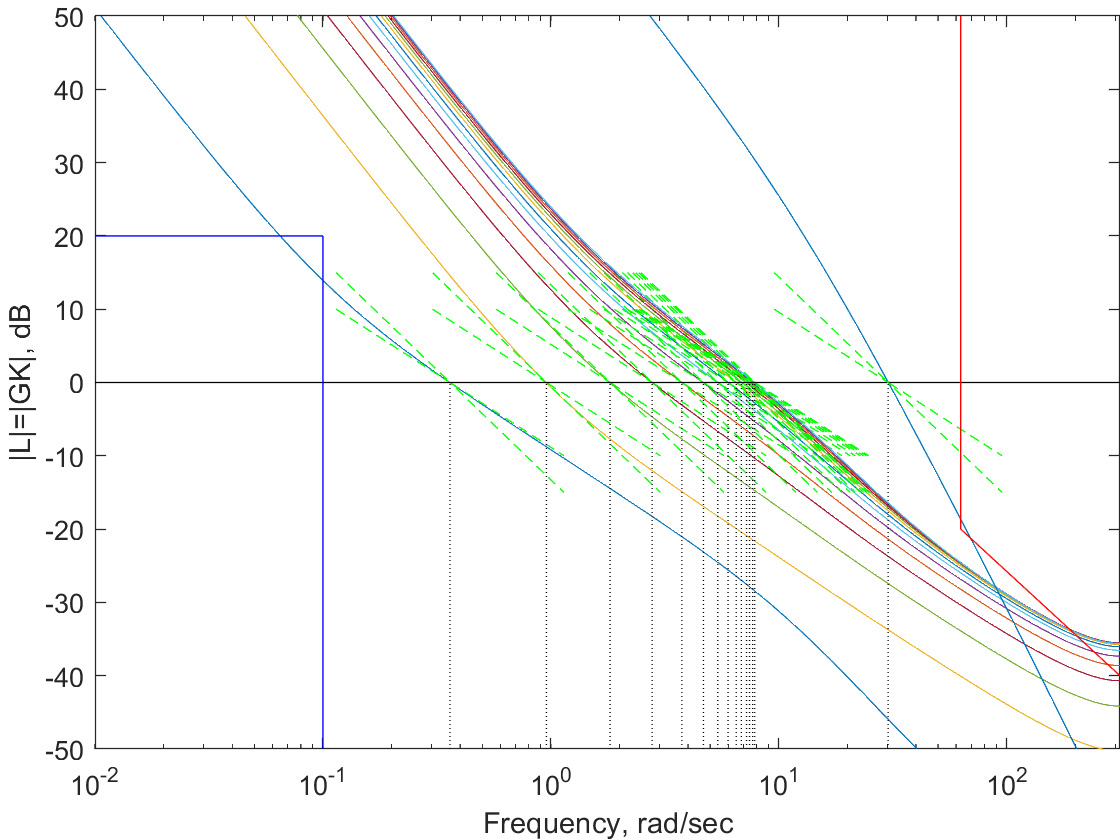
\includegraphics[width=0.7\linewidth]{images-design/controller_loopshape.png}
    \caption{Loopshape of open rocket $\to$ controller loop}
    \label{fig:controller_loopshape}
\end{figure}

\subsection{Optimal control theory}
\label{sec:controller-theory}
\textit{This section is here for completeness, it is not relevant for implementation.}
The LQR method uses the weighting matrices $Q$ and $R$ to solve the linear quadratic optimization problem \cite{werner2021b} \footnote{I think this came out better than the estimation theory, please be kind Prof. Werner, Prof. Faulwasser}
\begin{equation}
    \min V = \int_0^{\infty} (x^T(t) Q x(t) + u^T(t) R u(t)) dt
\end{equation}
for which the solution is of the form 
\begin{equation}
    V^* = x^T P x
\end{equation}
In infinite time, $P$ satisfies the algebraic Ricatti equation 
\begin{equation}
    PA + A^TP - PBR^{-1}B^TP + Q = 0
\end{equation}
which results in the control law
\begin{align}
    u^*(t) &= K x(t) \\
    K &= -R^{-1}B^TP
\end{align}
The resulting controller for the linear system is optimal in the trade-off of minimizing the state error $x(t)$ and control effort $u(t)$ \cite{werner2021}.
The closed-loop is guaranteed to be stable \cite{werner2021b}, and has margins of $[\infty, 0.5]$ in gain and $60^\circ$ in phase. 
This guarantee is only valid however for linear systems with full state measurements \cite{doyle1978}.
The control law is still useful for controlling nonlinear and observed systems, as the robustness properties can be partially preserved \cite{werner2021b}.

\subsection{Gain scheduling}
\label{sec:controller-scheduling}
As the models from canard angle to roll rate are nonlinear and highly dependent on some slowly-varying parameters (the \textit{flight conditions}), a gain-scheduling scheme will be implemented. 
This is common practice in aerospace applications dealing with different flight conditions \cite{theis2023}.
The design points $x_s$ of the schedule are characterized by these slowly-varying flight conditions $x_{FC} = \begin{bmatrix} \bar p & C_L \end{bmatrix}$, being the aerodynamic pressure $\bar p$, and the lift coefficient of the canards $C_L$. 
The simplified model is evaluated around these design points using the current state estimate $A(\hat x_{FC})$, to form the matrix $A$.
As the LQR method produces guaranteed robustness margins \cite{doyle1978, werner2021, werner2021b}, the  interpolation between two close design points should always produce a stable control loop.
\begin{figure}[ht]
    \centering
    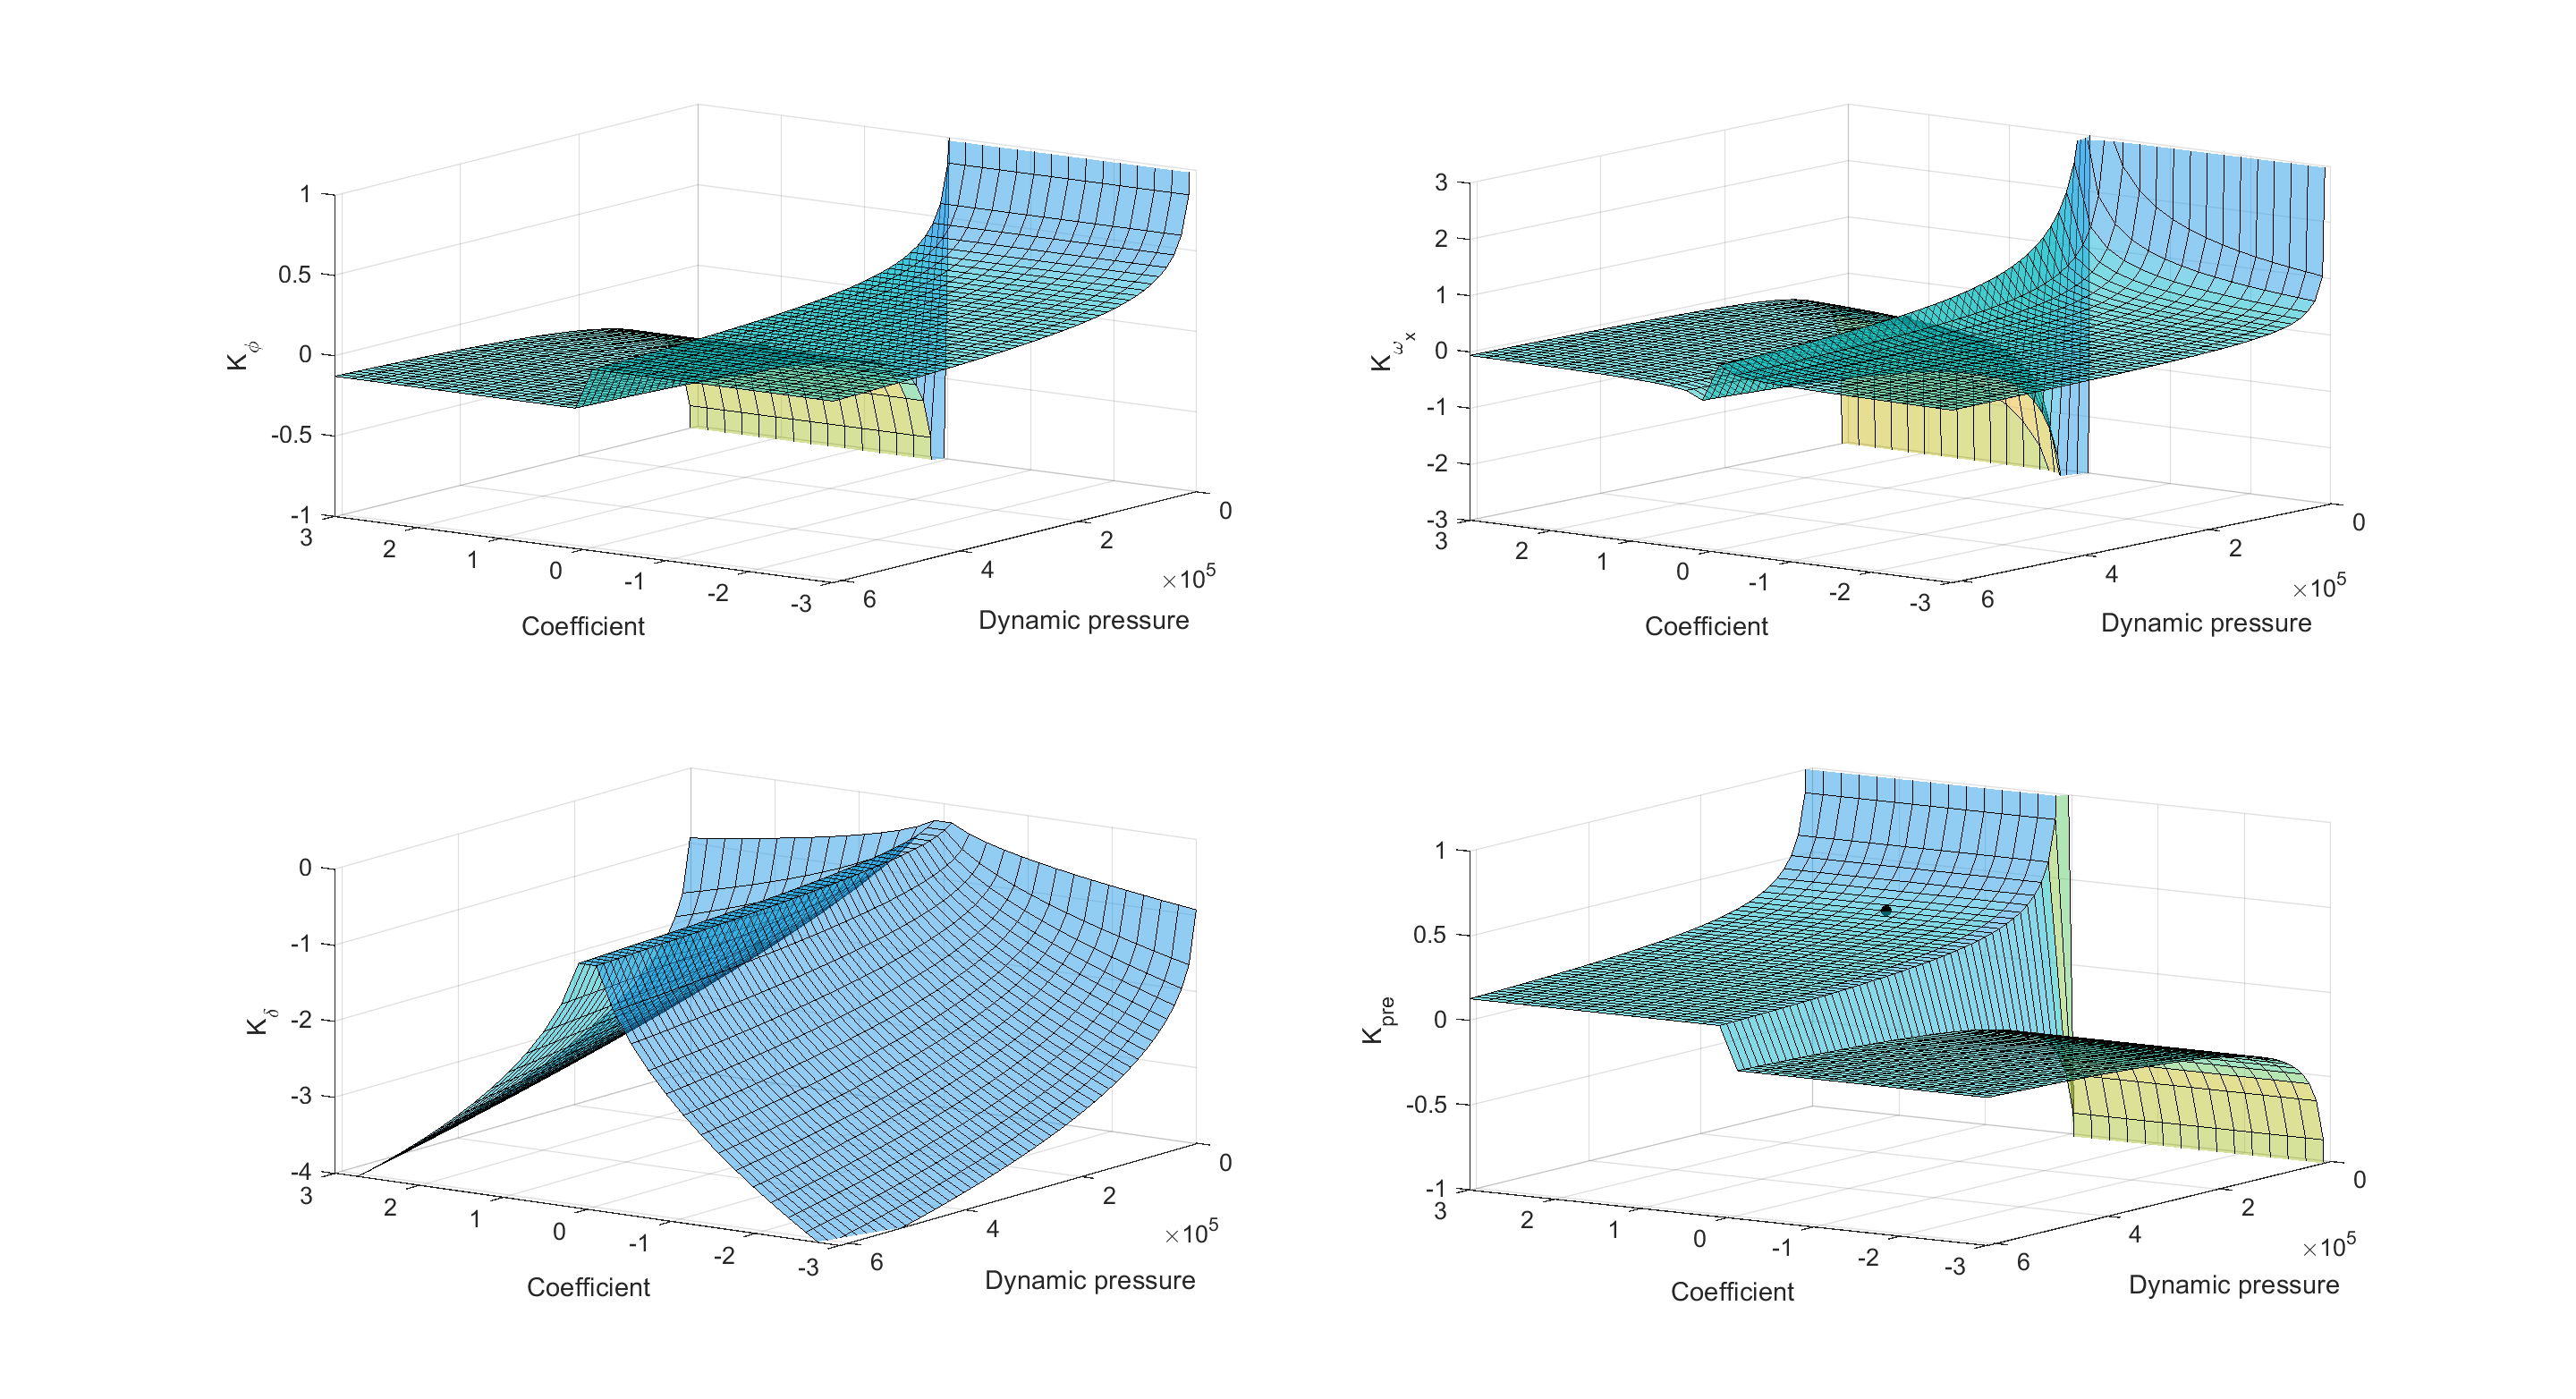
\includegraphics[width=0.95\textwidth]{images-design/controller_scheduling-surfaces.png}
    \caption[Scheduling surfaces along dynamic pressure and canard coefficient]{Scheduling surfaces along dynamic pressure $\bar p$ and canard coefficient of lift $C_L$. Feedback gains $K_\phi, K_p, K_\delta$ and reference gain $K_\textit{pre}$.}
    \label{fig:controller-surfaces}
\end{figure}

A large variety of design points are chosen, both along the nominal flight profile, but also encompassing a larger flight envelope to accommodate off-nominal trajectories.
Design points for the condition $L_\delta = 0$ are omitted from the tuning process, as the system is not controllable there.
The control gains for all design points are computed beforehand and stored in a look-up table.
In flight, the control algorithms interpolate the gains from the look-up table according to the current state estimate. 
The pre-computed feedback gains for the roll model are shown in Figure \ref{fig:controller-surfaces}, plotted over the scheduling variables $\bar p$ and $C_L$.
To note is the discontinuity at $\bar p = 0$ and especially at $C_L = 0$, where no feasible design points exist. 
The feedback gains are interpolated over this split.


\subsection{Response analysis}
To analyze some aspects of the control loop, the closed-loop responses are analyzed.
The closed-loop is technically a sampled-data system, with continuous time (the rocket) and discrete time (estimator and controller) dynamics.
For a high sampling rate (short time periods between control outputs), the discrete-time and the continuous-time closed-loop are approximately equal. 
The continuous-time dynamics are (from Equation \ref{eq:controller-closedloop})
$ \dot x_R = (A+BK) x_R + B K_{pre} r$ and $ y_R = C x_R $, with $C = \begin{bmatrix} 1 & 0 & 0 \end{bmatrix}$ for the $r \to \phi$ channel.

The weighting matrices are chosen as 
\begin{align}
    Q_c &= \begin{bmatrix}
        10 & & \\ & 1 & \\ & & 10  
        \end{bmatrix}
    &
    R_c &= (1 \cdot 10^{-3})\,  \bar p
\end{align}

The closed-loop step response for a collection of parameters (here varying velocities) is shown in Figure \ref{fig:controller-steps}.

\begin{figure}[ht!]
    \centering
    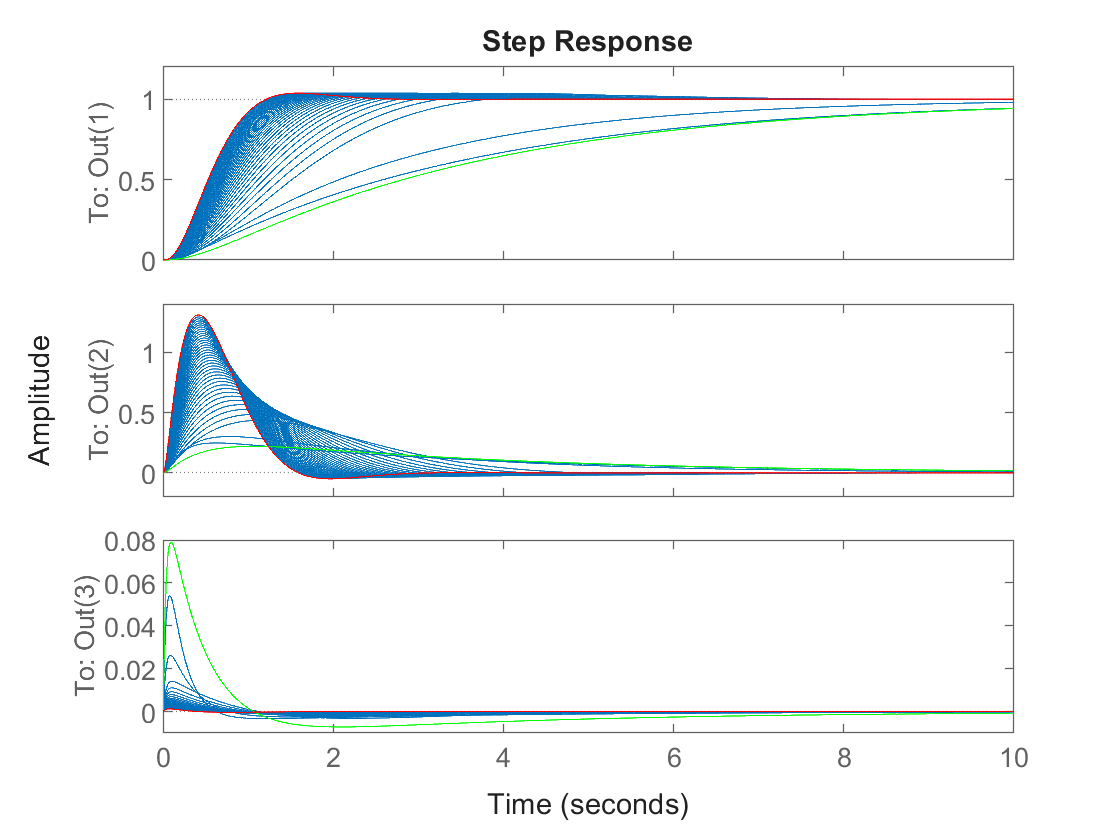
\includegraphics[width=0.8\textwidth]{images-design/controller_steps.png}
    \caption[Closed-loop step responses]{Step responses of the closed-loop system for velocities between $30\mathrm{m/s}$ (green) and $800\mathrm{m/s}$ (red), $l=1000\mathrm{m}$, $C_L = 1.5$. Outputs: 1:$\phi$, 2:$\omega_x$, 3:$\delta$.}
    \label{fig:controller-steps}
\end{figure}

The Bode plots of the closed-loop for a collection of parameters (here varying velocities) is shown in Figure \ref{fig:controller-bodes}.

\begin{figure}[ht!]
    \centering
    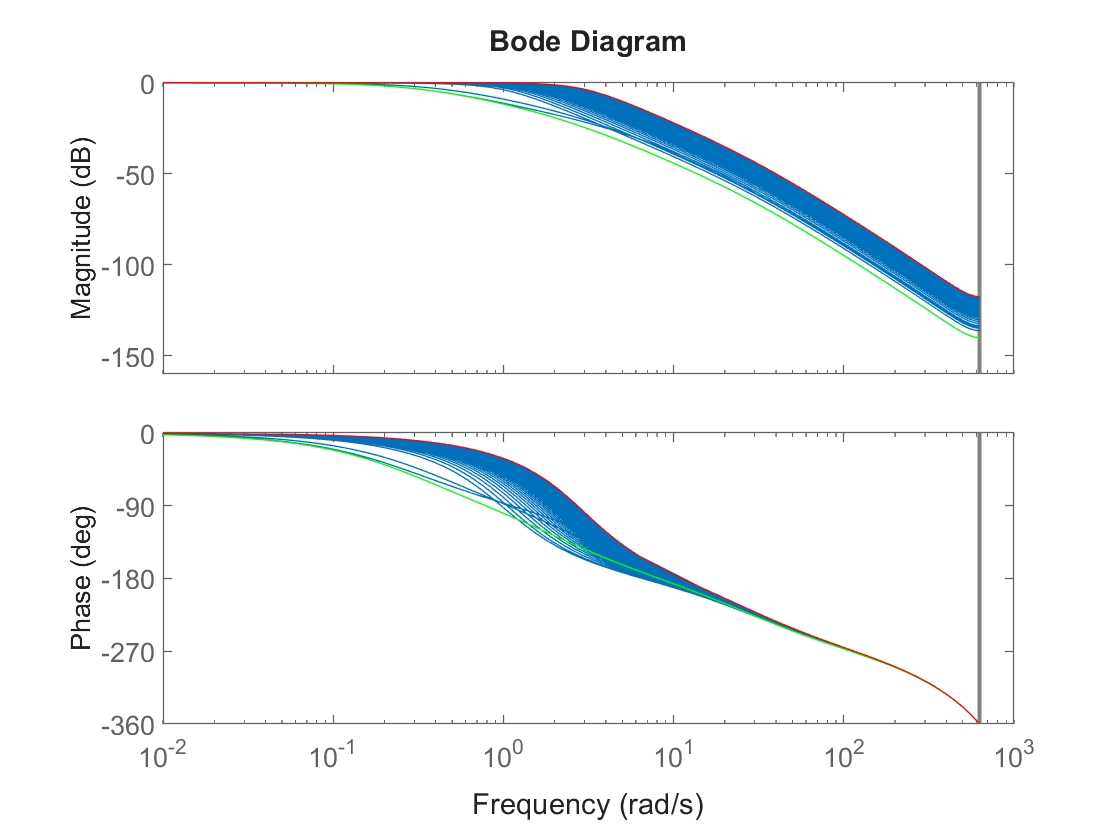
\includegraphics[width=0.8\textwidth]{images-design/controller_bodes.png}
    \caption[Closed-loop frequency response]{Frequency response of the closed-loop system for velocities between $30\mathrm{m/s}$ (green) and $800\mathrm{m/s}$ (red), $l=1000\mathrm{m}$, $C_L = 1.5$.
    The response is cut off above the sampling frequency of the processor.}
    \label{fig:controller-bodes}
\end{figure}


